\documentclass[a4paper, twocolumn, DIV=15]{scrartcl}
\usepackage[T1]{fontenc}
\usepackage[utf8]{inputenc}
\usepackage[british]{babel}

\addtokomafont{disposition}{\rmfamily}
\addtokomafont{descriptionlabel}{\rmfamily}

\usepackage{amsmath}
\usepackage{amssymb}

\usepackage{todonotes}

\usepackage{booktabs}
\usepackage{hyperref}

\usepackage{minted}
\usemintedstyle{solarizedlight}
\usepackage{mdframed}
\surroundwithmdframed{minted}

\usepackage{wrapfig}

\setminted[c++]{fontsize=\footnotesize}
\setminted[glsl]{fontsize=\footnotesize}

\usepackage[sorting=none,style=numeric]{biblatex}
\bibliography{references}

\renewcommand{\vec}[1]{\mathbf{#1}}
\newcommand{\hvec}[1]{\mathbf{\tilde #1}}
\newcommand{\norm}[1]{\left\Vert #1 \right\Vert}

\DeclareMathOperator*{\argmin}{arg\,min}

\title{\huge Particle System Using Instancing\\
    \normalfont \Large Project in Computer Graphics (1TD388) -- Spring 2018}

\author{Per Engström \and Jesper Middendorff \and Rasmus Précenth}

\date{\today}

\begin{document}

\maketitle

\thispagestyle{empty}

\section{Introduction}
\label{sec:introduction}

Particle systems is a method used in computer graphics to create
effects such as fire, smoke, sparks and fog. First introduced in the
1983 movie \emph{Star Trek II -- The Wrath of Khan}~\cite{reeves1983}
they are now abundant in both video games and movies.

This project displays one particular method of rendering a particle
system, using something called instancing. Instancing is a way to draw
many copies of the same geometry, but only sending it once to the
GPU. The alternative, sending the same geometry once for each
particle, is much slower. The particles are then rendered
back-to-front as billboards and blended to give the final result.

\section{Our approach}
\label{sec:our_approach}

The system implemented in this project is based on the particle system
tutorial in \cite{opengl-tutorial} with an additional GUI to tune the
parameters of the system.

Each particle in the system is rendered using billboarding by putting
a quad in front of the camera. The vertex shader receives the quad
vertices; the particle position, colour and time-to-live; and the
camera up and right vectors. This makes it possible to compute the
billboard position from just a single position per particle instead of
four and thus make a performance saving of 75\%.

\begin{minted}{glsl}
vec3 particle_vert = particle_pos
                   + up * billboard_vert.y
                   + right * billboard_vert.x;
\end{minted}

But it is possible to create an even bigger performance boost.
\emph{Instancing} is the concept of creating geometry once and reusing
it multiple times. In OpenGL it is acheived by binding data to the
buffers with \texttt{glBindData}, enabling a generic vertex attribute
array with \texttt{glEnableVertexArrayAttrib} and then pointing to the
data with \texttt{glVertexAttribPointer}.
\begin{table}[!h]
  \centering
  \begin{tabular}{r c c l}
    Buffer & Size & Step & Elements \\
    \hline
    Quad & 1 & 0 & $q$ \\
    Position & $n$ & 1 & $p_{0},p_{1},\dots,p_{n-1}$ \\
    Colour & $n$ & 1 & $c_{0},c_{1},\dots,c_{n-1}$ \\
    Time-to-live & $n$ & 1 & $l_{0},l_{1},\dots,l_{n-1}$ \\
  \end{tabular}
  \caption{Vertex attribute arrays.}
  \label{tab:buffers}
\end{table}

\begin{wrapfigure}{R}{0.2\columnwidth}
  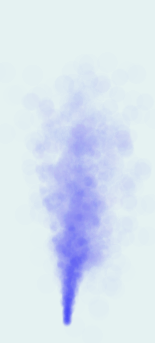
\includegraphics[width=0.2\columnwidth]{smoke}
\end{wrapfigure}
A step size (``divisor'') needs to be set for each array which
controls how the pointers advance through the attribute arrays. For
the quad the step size is set to 0 since it is reused for every
particle. All other arrays get a divisor of 1, see Table
\ref{tab:buffers}.

Finally, the particles are alpha blended together to create the final
results. It is important to sort the particles in decreasing order
according to their distance to the camera to produce a proper blend.

\printbibliography

\end{document}
